\documentclass[border=3pt]{standalone}
% Preâmbulo compartilhado pelos diagramas TikZ da aula 7 (Filtros Não Paramétricos)
\usepackage[T1]{fontenc}
\usepackage[utf8]{inputenc}
\usepackage{lmodern}
\usepackage{amsmath}
\usepackage{xcolor}
\usepackage{tikz}
\usetikzlibrary{arrows.meta,angles,quotes,decorations.pathmorphing,calc,
                positioning,shapes.geometric,shapes.misc,backgrounds,fit,
                math}

% Paleta (mesma dos SVGs originais)
\definecolor{dblue}{HTML}{2A5B8C}
\definecolor{dorange}{HTML}{B3541E}
\definecolor{dgreen}{HTML}{4A7C59}
\definecolor{dred}{HTML}{9C4B4B}
\definecolor{dcream}{HTML}{F4F1EA}
\definecolor{dshade}{HTML}{DDD7C9}

% Função gaussiana (não normalizada por padrão de escala visual)
\pgfmathdeclarefunction{gauss}{3}{%
  \pgfmathparse{1/(#3*sqrt(2*pi))*exp(-((#1-#2)^2)/(2*#3^2))}%
}

% Estilos comuns (prefixo d... para não colidir com chaves internas do pgf)
\tikzset{
  >={Stealth[length=2mm]},
  dguide/.style={gray!55, dashed, line width=0.4pt},
  daxis/.style={gray!60, line width=0.7pt, ->},
  dbody/.style={fill=black!3, draw=black!80, line width=1pt},
  dacc/.style={draw=dblue, line width=1pt},
  dlbl/.style={black!55, font=\small},
  dsub/.style={black!45, font=\footnotesize},
  dstate/.style={circle, draw=black!80, fill=dcream, line width=1pt,
                 minimum size=17mm, font=\large, inner sep=1pt},
  dobs/.style={circle, draw=black!80, fill=dshade, line width=1pt,
               minimum size=14mm, font=\large, inner sep=1pt},
  dbox/.style={rounded corners=2pt, draw=black!80, fill=dcream, line width=1pt,
               align=center, inner sep=6pt},
  dop/.style={circle, draw=black!80, fill=white, line width=1pt,
              minimum size=6mm, inner sep=0pt, font=\small},
  dtrans/.style={->, dblue, line width=1pt},
  dmeas/.style={->, dorange, line width=1pt},
  dcurve/.style={line width=1pt, dblue},
  dcurveb/.style={line width=1.4pt, dorange},
}

\begin{document}
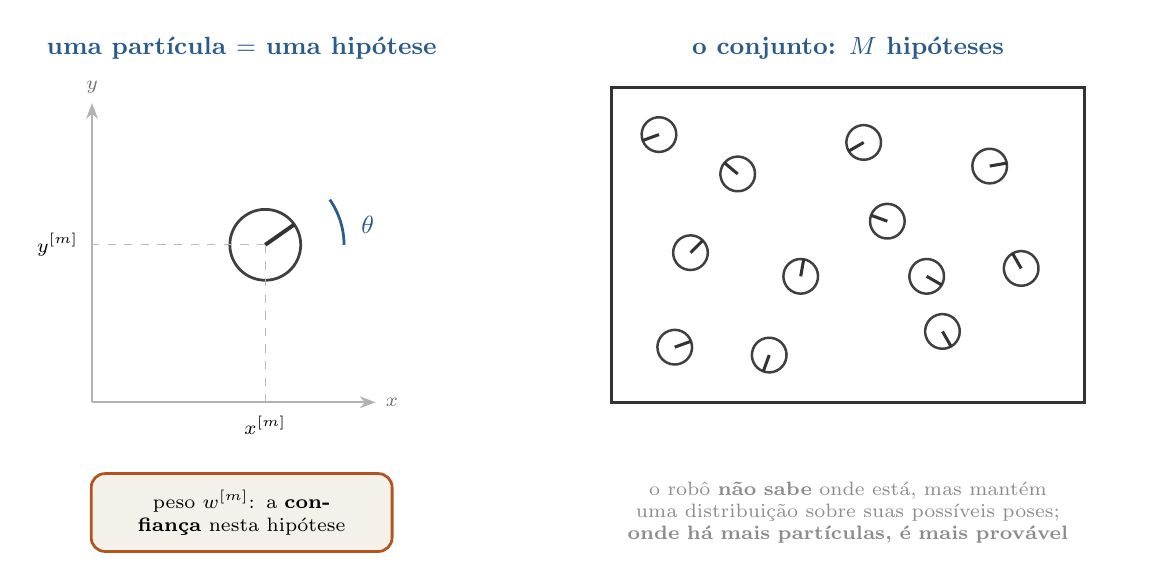
\begin{tikzpicture}[x=1cm,y=1cm]
  \newcommand{\rob}[4]{\begin{scope}[shift={(#1,#2)}, rotate=#3] \draw[black!75, fill=white, line width=1pt] (0,0) circle (#4); \draw[black!80, line width=1.4pt] (0,0) -- (#4,0); \end{scope}}
  % uma partícula
  \draw[black!30, line width=0.6pt, dashed] (0,0) -- (3.2,0); \draw[black!30, dashed] (0,0) -- (0,3.4);
  \draw[daxis] (0,0) -- (3.6,0) node[right, dlbl, font=\scriptsize] {$x$}; \draw[daxis] (0,0) -- (0,3.8) node[above, dlbl, font=\scriptsize] {$y$};
  \rob{2.2}{2.0}{35}{0.45}
  \draw[dguide] (2.2,2.0) -- (2.2,0); \draw[dguide] (2.2,2.0) -- (0,2.0);
  \draw[dblue, line width=1pt] (2.2,2.0) ++(1.0,0) arc (0:35:1.0); \node[dblue, font=\small] at (3.5,2.25) {$\theta$};
  \node[font=\scriptsize, anchor=north] at (2.2,-0.05) {$x^{[m]}$}; \node[font=\scriptsize, anchor=east] at (-0.05,2.0) {$y^{[m]}$};
  \node[dbox, rounded corners=5pt, draw=dorange, font=\scriptsize, text width=3.4cm] at (1.9,-1.4) {peso $w^{[m]}$: a \textbf{confiança} nesta hipótese};
  \node[font=\small\bfseries, dblue] at (1.9,4.5) {uma partícula $=$ uma hipótese};
  % conjunto
  \begin{scope}[shift={(6.6,0)}]
    \draw[dbody, fill=white, line width=1pt] (0,0) rectangle (6,4.0);
    \foreach \x/\y/\a in {0.8/0.7/20,1.6/2.9/140,2.4/1.6/80,3.2/3.3/210,4.2/0.9/300,1.0/1.9/45,3.5/2.3/160,2.0/0.6/250,4.8/3.0/10,5.2/1.7/120,4.0/1.6/330,0.6/3.4/200} { \begin{scope}[shift={(\x,\y)}, rotate=\a] \draw[black!75, fill=white, line width=0.9pt] (0,0) circle (0.22); \draw[black!80, line width=1.1pt] (0,0) -- (0.22,0); \end{scope} }
    \node[font=\small\bfseries, dblue] at (3,4.5) {o conjunto: $M$ hipóteses};
  \end{scope}
  \node[dsub, font=\scriptsize, align=center, text width=7cm] at (9.6,-1.4) {o robô \textbf{não sabe} onde está, mas mantém uma distribuição sobre suas possíveis poses; \textbf{onde há mais partículas, é mais provável}};
\end{tikzpicture}
\end{document}
